\subsection{Line and Corner Point Detection}

This year the algorithm used in previous years to detect field lines and corners  [Quinlan \emph{et al.}, 2006] was ported from the Aibo to the new Nao system. This required rewriting the function that transforms the found corner points in the camera plane to the field plane to suit the new robot kinematics and camera perspective. Otherwise, the algorithm is the same as the previous years for detection. Further development this year involved uniquely identifying these found corner points for use in Localization.

\subsubsection{Line Detection}
The detection of field lines is approached in a completely different manner to that of other Objects. When searching for objects, sections of a specific colour are joined together to form a blob. While this works well for most objects, white causes problems due to its abundance in the image and hence is normally ignored. Also the thin nature of lines, and the robot's low Point Of View, makes missing pixels very common within the classified image. Finally the storing of blobs, as a square which bounds the entire object, does not store enough important information about the line.

To overcome these issues the detection of lines is based around the two unique features that field lines have; their long thin length and their green-white-green transitions. Using these two details the image can be sparsely searched, since the search line does not need to find every point of the line, just enough to re-create the line. Also the transition information allows many white pixels to be thrown out early in the detection process, thereby reducing the overall load on the processor. This reliance on points and not the entire line also allows the lines to be partially hidden behind another object without effecting their detection. 

With these factors in mind, the image can now be efficiently searched in the following steps;

\begin{itemize}

\item 	The image is searched using a horizontal and vertical search grid. The search is restricted to the area in the image below the horizon line and picks out points of sharp contrast which have green-white then white-green transitions. These points are recorded in an array for later use.

\item The found points are then checked against each other to form possible lines. Once candidates are found, more points are checked and added until a line is formed. All checks on the lines at this stage is done based on gradient to allow the fastest line formation.

\item The lines are cleaned up to make sure all points actually fit on the line. Lines which have too large a number of points not contained within the final line are removed.

\item Lines are checked against each other to confirm that they are not just segments of larger lines. The allows lines to be formed that have a break in the middle, such as when a robot is on top of the line.

\item Corner points are found by extending lines and finding their intersection locations. The intersections are checked to confirm virtual points are not found. 

\item An attempt is made to uniquely identify corner points from other objects within the image. While this is not always needed, if a unique identification is made the use of the corner point within localisation becomes much more efficient.

\end{itemize}

\subsubsection{Corner Point Detection}
The locating of these corner points alone in each frame is not enough to localize with as there are numerous type-L and type-T corners on each side and a complete mirror image of the field lines on each half end of the field. Unique identification of each corner point is required in our system. A rule based approach was used to perform this identification that filters out the possible corner identity based on what properties of the corner can be extracted from the image and in most cases also some vague knowledge of robot location and orientation. 

The goal was not to provide data that Localization can rely upon solely but to fine tune the accuracy once approximate localization has been established. However this use of knowledge of location and orientation creates a loop between the Line Detection and Localization system components. This allows for the possibility of each component validating each other's incorrect data to exist. This being the case, the main focus was to write identification rules that are strict enough to eliminate the possibility of false positives. Also, the corner point identification rule written would block (that is, return an unknown corner or T point) unless the Localization confidence first came within 2 standard deviations of the probable orientation.
      
The identification relies upon the orientation of the seen corners, the combination of these corners and other lines in the image and the number of corners and lines seen. The Line Detection algorithm classifies each corner as either a type L or T and then attributes it with one of four possible orientations, pointing up/down or pointing left/right. By disassembling the field lines in the image they could be examined for what types of corners and orientations make up what is seen. Following that, this information is then decoded to match what should be seen from the present known location. Avoiding false positives here partially takes care of itself as if the robot location or orientation data is wrong, the corresponding corner orientation classification will not match the rule.

For example, in Figure \ref{fig:corner}a taken from the simulator, the detection algorithm reports seeing 3 corners: 2 type L's of orientation 2 and 4, 1 type T of orientation 1 and 4 lines. This set of data is almost unique when compared to the other countless possible positions and perspectives from which to view the field lines and can therefore be decoded with brute force. 
 
The only other occurrence is a duplicate on the opposite end of the field as both halves are identical. This the leaves the question, "which end of the field is the robot in?". Knowledge of the robots orientation could also solve this problem of determining which end of the field this scene is taken from. To be robust, the rules written require Localization to be certain of both field XY position and orientations to 2 standard deviations. This value could be increased in this case but for others closer to the mid field line, the probability of error increases as the two mirror images from each end come closer together. The necessity for this prior knowledge is best show pictorially.
    
In the first frame we have no other information to work with other than the lines themselves. In the second frame, the Goal Detection provides Localisation with enough information to determine which end of the field the robot is in and it is now possible to uniquely identify the corner points.
      
Another example of an identification rule would the identification of a mid field T corner. Conditional tests for seeing only: 2 field lines, corner count = 1, corner type = T, corner orientation = 3, robot X location is greater than zero, orientation is 135 degrees plus or minus 80 degrees and no goal post is seen, accurately reports the correct corner and filters out all others.
      
Unique identification rules were written for each corner for a selection of possible perspectives and rigorously tested in the Webots simulator. Possible sources of error discovered in testing were the extension of the penalty box line to join the side field line to create a phantom type T corner, the clipping of a type T corner into a type L by the edge of the camera frame and the center circle appears as a collection of many corners (for example an octagon). Each of these sources of error were reliably filtered out by the corner combination decoding.
      
The simulation testing also showed great improvement in Localisation over simply relying upon goal detection alone. Once a goal had been seen and Localisation determined to some approximate area, the line detection would report a unique corner point and fix a very accurate position and orientation and maintain it while looking all around the field. 

The identified point on the field is then sent to Localization after performing the following transformation.

$V_{cam}=[focLength, (IMG_{width}/2)- X_{img},(IMG_{height}/2)-{Y_{img}}]$

Transformation through neck

\textbf{$V_{1}$}=\textbf{$V_{cam}$}*\textbf{$M_{camTilt}$}

\textbf{$V_{2}$}=\textbf{$V_{1}$}*\textbf{$M_{camPan}$}

Transform body tilt

\textbf{$V_{3}$}=\textbf{$V_{2}$}*\textbf{$M_{bodyTilt}$}

$\alpha=-Chest Height/V_{3}[2]$

$distance=\alpha*\sqrt{V_{3}[0]^2+V_{3}[1]^2}$

$bearing=arctan2(V_{3}[0],V_{3}[1])$

This inter system approach to the corner identification is shown in Figure \ref{fig:corner} b and c. Green components demonstrate an improvement to this approach where one of the Localisation reset triggers becomes an external one based on an added component that monitors for robot relocation by hand by way of accelerometer readings (Teleport Detection if image is BW). In the Robocup competition robots do get picked up and moved, possibly to the other side of the field and turned around by 180 degrees when being penalized. The loop created between the Line Detection and Localisation could slow down the reset as it would take some time for the bad data to be dumped after locating a goal post and dealing with conflicting information. A specialised system component could ensure this does not happen.
\begin{figure}[htpb]
\begin{center}
    %\leavevmode
    \scalebox{0.3} {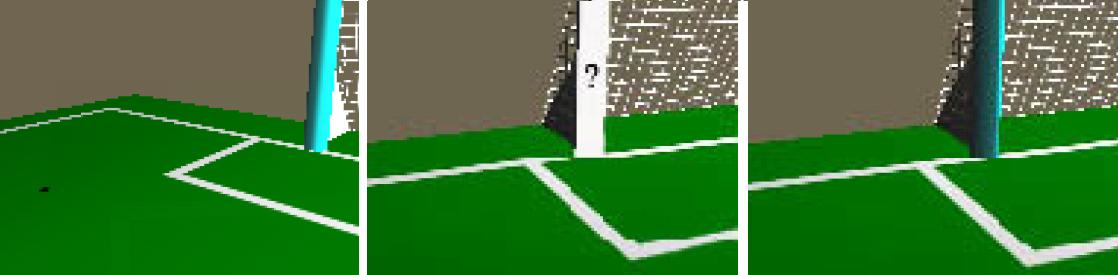
\includegraphics{alexfigs/corner.png} }
    \caption{Images of corners for examples.}
    \label{fig:corner}
\end{center}
\end{figure}

%\subsubsection{Code Implementation}
%Up until this year, Line Detection was a collection of functions within the Vision class itself. To
%reduce coupling, the Line Detection function and supporting functions were removed from the vision
%class and placed into a newly created Line Detection class. This Line Detection class is responsible for
%both line detection and the corner identification. These routines are still part of the vision system and
%the files can be found in the vision directory. No other NUManoids system component is dependent
%upon this Line Detection class to in order run and therefore it may be removed from the project build by
%editing the MakeFile in the root of the code body.
%Once a Line Detection object has been instantiated, the Line Detection function �formlines()� is
%called at the end ProcessFrame() within the class Nao. It requires no data to be passed into it and it
%outputs its results by directly modifying the elements found in the �fieldObjects� structure. The list of all
%possible corner points that can be evaluated can be found in the FieldObject.h file.
%\begin{figure}[!ht]
%\begin{center}
%    %\leavevmode
%    \scalebox{0.3} {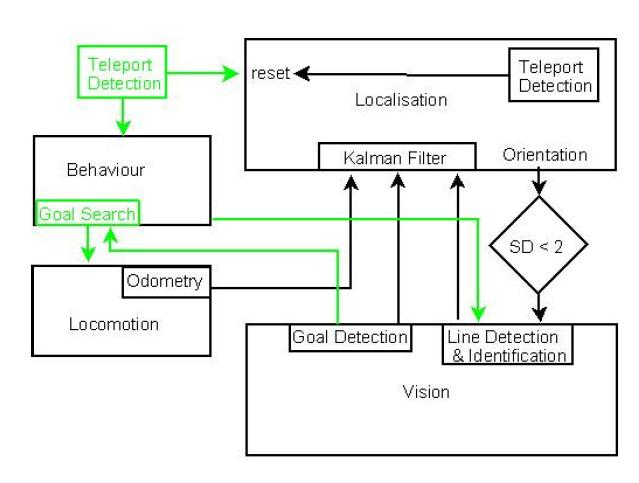
\includegraphics{alexfigs/flow.png} }
%    \caption{Software flow diagram.}
%    \label{fig:flow}
%\end{center}
%\end{figure}


\subsubsection{Penalty Spot Detection}
Penalty spots exists in two positions on the field. By detecting any penalty spot, localisation module has a higher chance of knowing where the robot is currently situated on the field. Detecting the penalty spot consists of a search heuristic:
\begin{itemize}
\item Find lines that are less then a quarter length of the screen: If a standing robot should see a penalty spot, it should be relatively small on the screen.
\item Using the points on the selected line, we scan around each of these line points for surrounding white colours:
This scan consists of a 3x3 grid search around the selected point.
\item If there does not exist to be any white colours, its most likely to be a penalty spot, Otherwise it is not a penalty spot.
\end{itemize}
This is a simple and efficient heuristic, because the priori conditions make the search space is very small.

\subsubsection{Centre Circle Detection}
Centre circle is an a very important field object on the SPL field. This object is so big that almost from any section of the field (provided that is facing inwards). It enhances and assists the localisation module greatly, due to its visibility and unambiguous properties of the object. To detect a centre circle, there exists two steps. First Step, is to remove points that do not belong on the centre circle. Second step, consists of an least squares approach to fit the points of the centre circle to an ellipse equation.
Once this is complete, we are able to obtain the ellipse, and the robots current distance to it.

The first step is removing points that do not belong on the centre circle, this is achieved by an heuristic. Here we assume that after all points have been fitted to a line, corners (intersections) of lines have been calculated and all penalty spots have already been detected. Here we assume a centre circle consists of many small straight lines, with many straight lines these should intersect on screen a large number of times. Assuming a number of corner tolerance of six, if the number of corners are greater then six, centre circle detection will be triggered. 
\begin{itemize}
\item Find the longest line (most likely to be the centre line) and remove it from the search list.
\item Find the Penalty Spot lines and remove it from the search list.
\item Assuming that the lines are small, we select all the small lines. For our system, a small line is a line that is less then half the image width.
\item We then select the line points that exist within these lines and store them in a vector ready to be processed by the next stage.
\end{itemize}

The next stage consists of fitting the obtained points to an ellipse equation. By fitting the points to an equation we are able to generalise and efficiently store the data of the ellipse for later use. The ellipse fitting algorithm is an C++ implementation of the Matlab version by Halif and Flusser. A summary and Matlab version of the algorithm is as follows in \autoref{fig:MatlabEllipseFitting} \cite{Halif98}.

\begin{figure}[htpb]
	\begin{center}
		{\scriptsize\begin{verbatim}
			1 function a = fit_ellipse(x, y)
			2 D1 = [x .� 2, x .* y, y .� 2]; % quadratic part of the design matrix
			3 D2 = [x, y, ones(size(x))]; % linear part of the design matrix
			4 S1 = D1� * D1; % quadratic part of the scatter matrix
			5 S2 = D1� * D2; % combined part of the scatter matrix
			6 S3 = D2� * D2; % linear part of the scatter matrix
			7 T = - inv(S3) * S2�; % for getting a2 from a1
			8 M = S1 + S2 * T; % reduced scatter matrix
			9 M = [M(3, :) ./ 2; - M(2, :); M(1, :) ./ 2]; % premultiply by inv(C1)
			10 [evec, eval] = eig(M); % solve eigensystem
			11 cond = 4 * evec(1, :) .* evec(3, :) - evec(2, :) .� 2; % evaluate a�Ca
			12 a1 = evec(:, find(cond > 0)); % eigenvector for min. pos. eigenvalue
			13 a = [a1; T * a1]; % ellipse coefficients
		\end{verbatim}}
		\caption{MatLab Code for Fitting points to an equation of an ellipse}
		\label{fig:MatlabEllipseFitting}
	\end{center}
\end{figure}
For the transition from Matlab to C++ a new library that enabled linear algebra calculations were included into the NUbot system. This linear algebra library was called 'JAMA' an adaptation for C++ of the Java Matrix Library available freely from \cite{JAMA}.

This was an efficient method of obtaining an equation of an ellipse with a small number of points, which we have filtered out to be ellipse points. 

\begin{figure}[htpb]
\begin{center}
    %\leavevmode
    \scalebox{1} {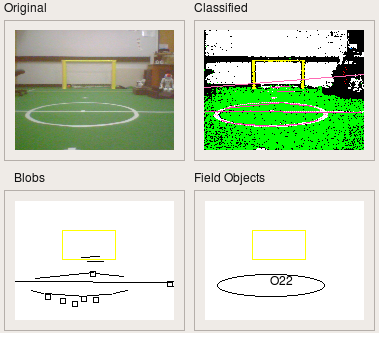
\includegraphics{aaronfigs/CentreCircleDetection.png} }
    \caption{The figure is taken from the debugging application EOTN mentioned earlier. Original Image: This is an image capture from the NAO robot. Classified Image: This image is an overlay of the horizon line, detected lines and classified image. Blobs: This displays the blobs and detected lines and corner points that are currently in the image. Field objects: shows the field objects detected in the image, here we see the result of fitting the points to an ellipse equation.}
    \label{fig:ellipse}
\end{center}
\end{figure}